\documentclass{article}

\usepackage{amsmath,amssymb}
\usepackage{tikz}
\usepackage{pgfplots}
\usepackage{xcolor}
\usepackage[left=2.1cm,right=3.1cm,bottom=3cm,footskip=0.75cm,headsep=0.5cm]{geometry}
\usepackage{enumerate}
\usepackage{enumitem}
\usepackage{marvosym}
\usepackage{tabularx}
\usepackage{multirow}

\usepackage[utf8]{inputenc}

\renewcommand*{\arraystretch}{1.4}

\newcolumntype{L}[1]{>{\raggedright\arraybackslash}p{#1}}
\newcolumntype{R}[1]{>{\raggedleft\arraybackslash}p{#1}}
\newcolumntype{C}[1]{>{\centering\let\newline\\\arraybackslash\hspace{0pt}}m{#1}}

\title{\textbf{Rechtfertigung der Staatstätigkeit, Hausaufgabe 5}}
\author{\textsc{Henry Haustein}}
\date{}

\begin{document}
	\maketitle
	
	\section*{Aufgabe 2}
	\begin{enumerate}[label=(\alph*)]
		\item Gesellschaftlich optimal wäre es, wenn die Grenzkosten gleich dem Grenzprodukt sind:
		\begin{align}
			GK &= GP \notag \\
			100 &= 200-10x \notag \\
			x^{opt} &= 10 \notag+
		\end{align}
		\item Ohne Zugangsbeschränkung bildet sich die Menge heraus, bei der Durchschnittsprodukt gleich Grenzkosten sind:
		\begin{align}
			GK &= DP \notag \\
			100 &= \frac{200x-5x^2}{x} \notag \\
			100 &= 200 - 5x \notag \\
			x^{priv} &= 20 \notag
		\end{align}
		\item Graph
		\begin{center}
			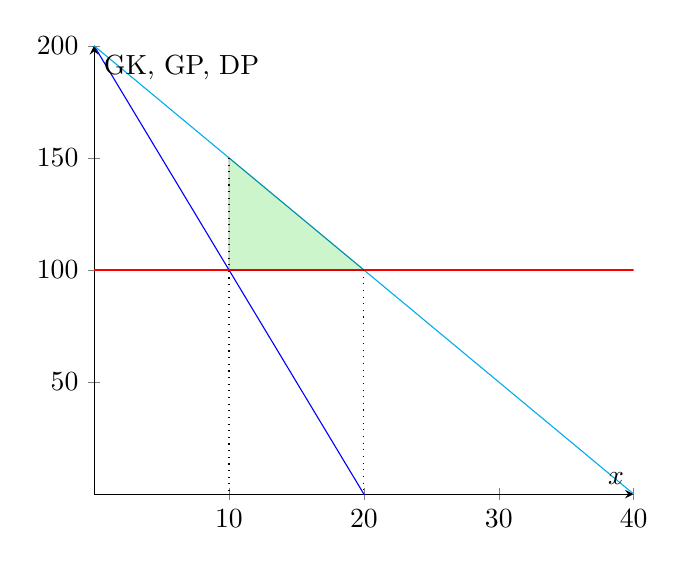
\begin{tikzpicture}
				\begin{axis}[
					xmin=0, xmax=40, xlabel=$x$,
					ymin=0, ymax=200, ylabel={GK, GP, DP},
					samples=400,
					axis x line=middle,
					axis y line=middle,
					domain=0:40,
					]
					\addplot[mark=none,smooth,blue] {200-10*x};
					\addplot[mark=none,smooth,cyan] {200-5*x};
					\addplot[mark=none,smooth,red] {100};
					
					\draw[dotted] (axis cs: 10,150) -- (axis cs: 10,0);
					\draw[dotted] (axis cs: 20,100) -- (axis cs: 20,0);
					
					\draw[fill=green!80!black,opacity=0.2] (axis cs: 10,100) -- (axis cs: 10,150) -- (axis cs: 20,100) -- (axis cs: 10,100);
					
				\end{axis}
			\end{tikzpicture} \\
			\textcolor{blue}{Grenzprodukt}, \textcolor{cyan}{Durchschnittsprodukt}, \textcolor{red}{Grenzkosten}, \textcolor{green!80!black}{Wohlfahrtsverlust}
		\end{center}
		\item Der Wohlfahrtsverlust ergibt sich zu
		\begin{align}
			\text{WFV} &= \frac{1}{2}\big[(DK(x^{opt}) - GP(x^{opt}))\cdot (x^{priv} - x^{opt})\big] \notag \\
			&= \frac{1}{2} \big[(150-100) \cdot (20-10)\big] \notag \\
			&= \frac{1}{2}\cdot 500 \notag \\
			&= 250 \notag
		\end{align}
		\item Der Preis sollte genau der externe Effekt im Optimum sein, dieser ist $DK(x^{opt}) - GP(x^{opt}) = 50$. Es sollten genau $x^{opt}=10$ Lizenzen verkauft werden, die Einnahmen betragen dann $50\cdot 10=500$.
	\end{enumerate}

\end{document}